\chapter{实验二:通信模型与参数聚合}

\section{实验内容与要点介绍}

\subsection{实验内容与要求}

\subsubsection{实验内容}
\begin{itemize}
    \item 了解并掌握分布式算法中的集体通信和参数聚合策略,了解并掌握集体通信中常用的消息传递接口(Reduce, AllReduce, Gather, AllGather, Scatter, etc.)
    \item 实现模型参数或模型参数梯度的聚合,尝试使用不同聚合方式(Sum, Mean, etc.)对模型的参数和梯度进行聚合,并分析不同聚合策略对模型性能的影响。    
\end{itemize}

\subsubsection{实验要求}
\begin{itemize}
    \item 实现集体通信下的参数/梯度聚合,基于至少2种集体通信原语实现梯度平均的聚合方法,并比较它们的通信时间开销
    \item 在框架下设置瓶颈节点,并讨论瓶颈节点对集体通信的影响
\end{itemize}

\subsection{多节点通信}

在本次实验中,我们采用PyTorch中的\graylstinline{torch.distributed}模块(下面将简写为\graylstinline{dist})作为多节点通信的支持工具。

\subsubsection{初始化进程组}

多节点通信的第一步,是初始化进程组。因此每个节点在训练之前,需要先调用\graylstinline{dist.init_process_group()}函数来初始化进程。这个函数会阻塞当前进程,并等待其他进程加入,阻塞持续至直到所有节点(进程)都加入了进来。

对于本次实验,我们需要关注这个函数的三个输入:\graylstinline{backend},\graylstinline{world_size}和\graylstinline{rank}。
\begin{itemize}
    \item \graylstinline{backend}指定通信后端,即实现多节点通信的底层的通信协议,对于本次实验,当在Linux环境下且使用GPU时,一般选择nccl,其他情况下,一般使用gloo即可(每种后端支持的设备类型和功能有所不同,更多内容可阅读官方文档\url{https://pytorch.org/docs/stable/distributed.html#backends})。
    \item \graylstinline{world_size}为进程总数。
    \item \graylstinline{rank}指定当前进程的优先级。启动多节点时,需要为每个进程指定rank,一般为每个进程赋值为0到进程总数-1中的整数。
\end{itemize}

但是光有这三个参数还不足以让多节点(进程)之间可以发现彼此,其实还需要告诉节点主进程的通信地址和端口。这里我们采用设置环境变量的方式告诉节点们如何找到\graylstinline{rank=0}的主节点。下面这段代码展示了\graylstinline{rank=0}的节点的初始化方式。
\begin{lstlisting}
    import torch.distributed as dist

    # change it to the corresponding ip addr
    os.environ['MASTER_ADDR'] = 'localhost'
    os.environ['MASTER_PORT'] = 12355
    
    # initialize the process group
    dist.init_process_group(backend="nccl", rank=0, world_size=2)
\end{lstlisting}

\subsubsection{广播模型参数}

完成进程组初始化后,在神经网络模型训练开始前,需要确保所有节点上的模型是一样的,因此需要将主节点上的模型的参数广播给其他所有节点。我们使用\graylstinline{dist.broadcast()}函数来同步所有节点的参数。

下面这段代码展示了广播过程,\graylstinline{dist.broadcast()}需要两个参数:
\begin{itemize}
    \item \graylstinline{tensor},为需要广播或接收的数据。当广播源为当前进程时,\graylstinline{tensor}将被发送给其他节点,当广播源不是当前进程时,\graylstinline{tensor}将被赋为接收到的数据。
    \item \graylstinline{src},为广播源的rank。
\end{itemize}

\begin{lstlisting}
    if get_world_size() > 1:
        for param in model.parameters():
            dist.broadcast(tensor=param.data,src=0)
\end{lstlisting}

\subsubsection{参数聚合}

神经网络模型训练过程中,就要实现参数聚合了。该部分请同学们自行完成。

\subsection{记录GPU上任务的运行时间}

利用\graylstinline{torch.cuda.Event.elapsed_time()}记录,示例代码如下:
\begin{lstlisting}
    start_evt = torch.cuda.Event(enable_timing=True)
    end_evt = torch.cuda.Event(enable_timing=True)
    start_evt.record()
    # the time between start_evt and end_evt will be caculated
    end_evt.record()
    torch.cuda.synchronize()
    whole_time = start_evt.elapsed_time(end_evt)
\end{lstlisting}

\section{使用进程模拟多节点}

为了模拟多节点通信,我们可以在同一台机器上使用不同进程或容器来实现。本节介绍多节点模拟的方法。通过进程模拟的方法在本地、在本地容器中、在华为云、在学校的计算平台都是通用的。

\subsection{手动运行多进程}
启动两个终端,分别指定不同的rank即可。例如:
\begin{lstlisting}[language=bash]
    # first process:
    $ python model.py --n_devices=2 --rank=0
    # second process:
    $ python model.py --n_devices=2 --rank=1
\end{lstlisting}

\subsection{使用torch.multiprocessing自动创建多进程}

通过\graylstinline{torch.multiprocessing}中的\graylstinline{spawn()}函数即可让该函数自动帮我们创建多个进程,其中,我们需要关注该函数的三个参数:
\begin{itemize}
    \item \graylstinline{fn}为函数名,将作为生成的进程的入口。
    \item \graylstinline{args}为tuple元组类型。每个进程将通过 \graylstinline{fn(i, *args)}的方式调用\graphicspath{fn},其中\graylstinline{i}即为所生成进程的rank,从0开始逐次递增1。
    \item \graylstinline{nprocs}为生成的进程总数,即前文所指的\graylstinline{worldsize}或\graylstinline{n_devices}。
\end{itemize}

下面一段代码简要说明了\graylstinline{spawn()}函数的使用方法。详情可参考\graylstinline{model-mp.py}。
\begin{lstlisting}
import torch.multiprocessing as mp
def main(rank, args):
    pass
if __name__ == "__main__":
    args = parse_args()
    mp.spawn(main, (args,), nprocs=args.n_devices)
\end{lstlisting}

\section{使用容器模拟多节点}

“容器就类似于虚拟机了,那通过容器模拟多节点岂不是更真实?”不知道有多少同学也和助教一样这样以为过。那我们就来尝试一下看起来更高端的容器模拟多节点吧。

注意,由于我们只在本地安装了docker并自定义了镜像(\S\ref{subsec:container-to-image}),所以下面的内容针对的是在本地使用容器模拟的过程。当然只要你掌握了方法,在远程的平台上也是一样使用的。

乍一看上去很复杂,多个容器之间的通信怎么处理呢?其实完全不用担心,我们只要使用docker compose就可以了,它会帮我们自动配置好同一组容器下的网络。

\subsection{Docker compose介绍}

我们以助教发给大家的\graylstinline{docker-compose.yml}为例,我们取其中的一部分先简单分析一下这个文件的内容。
\begin{lstlisting}
services:
    node01:           
        # container_name: node01
        image: cantjie/pytorch:1.13.1
        volumes:
          - .:/workspace      # <host(local) dir (should start with . or /)>:<dir in container>
        command:              # python /workspace/model.py --n_devices=1 --rank=0 --gpu=0
          - python
          - -u
          - /workspace/model.py 
          - --n_devices=2
          - --rank=0
          - --gpu=0
          - --master_addr=localhost
          - --master_port=12378
        deploy:              # make GPU accessible in container
          resources:
            reservations:
              devices:
                - driver: nvidia
                  count: 1
                  capabilities: [gpu]
\end{lstlisting}

文件中定义了两个\graylstinline{services},每个\graylstinline{service}就对应了一个容器,对于每个容器的配置,以\graylstinline{node01}为例,我们通过\graylstinline{image}指定了镜像,通过\graylstinline{volumes}指定了文件挂载路径(参考\S\ref{subsec:docker-run-and-mount-volume}),通过\graylstinline{command}指定了容器启动后需要执行的命令,下面这个写法实际上是告诉容器执行这条语句:
\begin{lstlisting}[language=bash]
    $ python -u /workspace/model.py --n_devices=2 --rank=0 --gpu=0 \
        --master_addr=localhost --master_port=12378
\end{lstlisting}
其中\graylstinline{-u}表示将Python中\graylstinline{print}命令的输出以unbuffer的方式输出,这是docker容器的一个特性,如果不加\graylstinline{-u},我们只能在训练完成、代码跑完之后才能看到程序输出的结果啦。

最后的\graylstinline{deploy}则是让容器能够使用宿主机的GPU(\graylstinline{deploy}这一段是网上复制来哒,细问我也不懂啦)。

至于\graylstinline{node02},除了\graylstinline{rank}外,只有\graylstinline{master_addr}与\graylstinline{node01}不同,对于\graylstinline{node01}来说,master就是自己了,而对于\graylstinline{node02}来说,master当然是\graylstinline{node01}了。

你可能要问,那为什么这里不是写master的ip,而是写“node01”就行了呢?这就是Docker compose的方便之处了,他会自动修改容器内的hosts,也就是“node01”就是\graylstinline{node01}这个节点的“域名”了。

\subsection{通过Docker compose启动容器}

将这个文件和\graylstinline{model.py}放到同一个目录下,然后终端\graphicspath{cd}到这里,输入\graylstinline{docker compose up}就完成啦,我们就可以看到程序已经开始训练了!如图\ref{fig:task2-docker-compose-up}所示。


\begin{figure}[htbp]
	\centering
	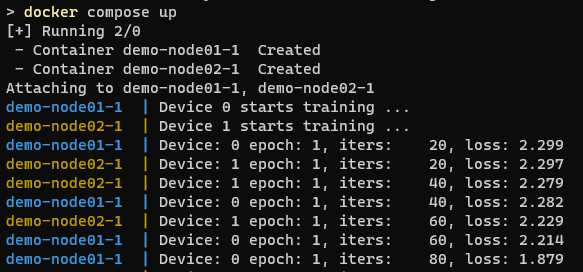
\includegraphics[width=0.7\textwidth]{figures/task2-docker-compose-up.png}
	\caption{caption:task2-docker-compose-up}
	\label{fig:task2-docker-compose-up}
\end{figure}

这里还需要注意的是,由于我们在yaml中,并没有使用\graylstinline{container_name}为容器指定名字,因此Docker生成容器的时候,会按照\graylstinline{<dir>-<service-name>-<number>}命名方式为我们的容器命名,如果你的\graylstinline{docker-compose.yml}处在一个中文名称的文件夹下,系统很可能会报错的。放到英文命名的文件夹下就好了。
